\subsubsection {Étape 3 : Téléchargez et configurez Apache Cassandra:}

\textbf{Télécharger et extraire le dossier Cassandra tar.gz}

\begin{enumerate}
\item Visitez la page officielle de téléchargement d'Apache Cassandra et sélectionnez la version que vous préférez télécharger. Actuellement, la dernière version disponible est 3.11.6.\href{https://cassandra.apache.org/_/download.html}{lien ici}
\begin{figure}[h]
	\centering
    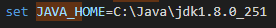
\includegraphics[scale=0.6]{img/part3/2.2}
    \caption{Site de téléchargement de Cassandra}
\end{figure}
\item Cliquez sur le lien de téléchargement miroir suggéré pour démarrer le processus de téléchargement.
\begin{figure}[h]
	\centering
    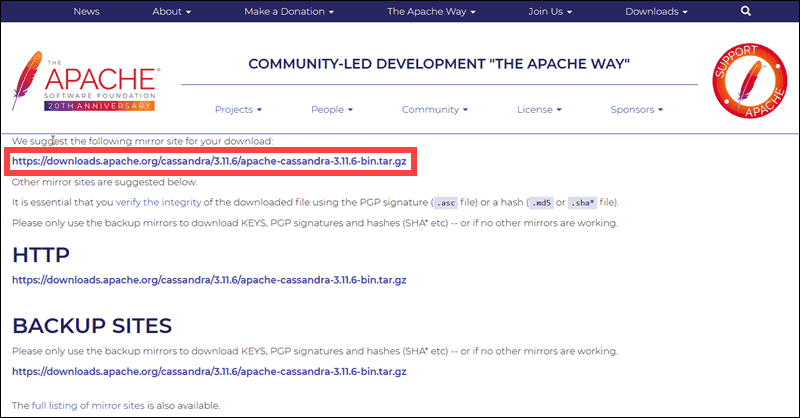
\includegraphics[scale=0.5]{img/part3/2.3}
    \caption{le lien de téléchargement miroir}
\end{figure}
\newpage
\item Décompressez le dossier tar.gz compressé à l'aide d'un outil de compression tel que 7-Zip ou WinZip. Dans cet exemple, le dossier compressé a été décompressé et le contenu placé dans le dossier C:/Cassandra/apache-cassandra-3.11.6.
\begin{figure}[h]
	\centering
    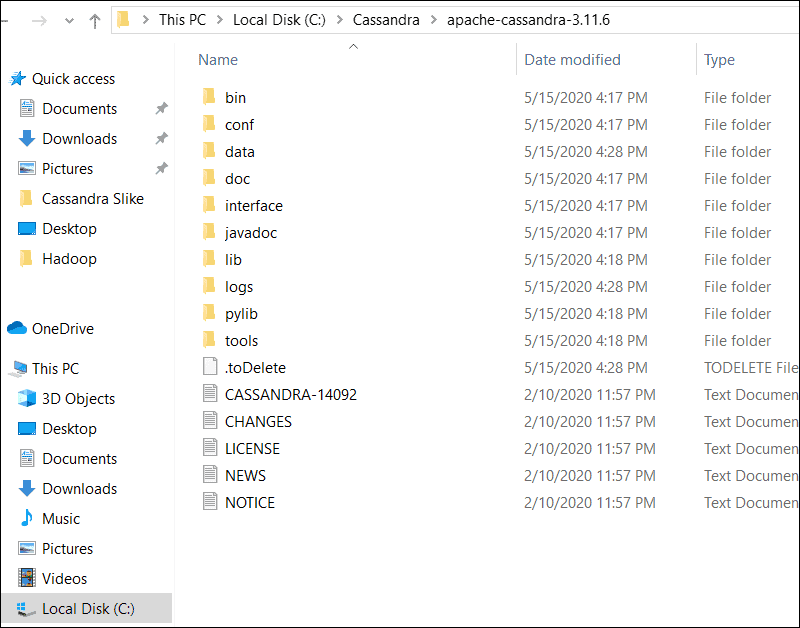
\includegraphics[scale=0.5]{img/part3/2.4}
    \caption{contenu du dossier}
\end{figure}
\end{enumerate}

\textbf{Configurer les variables d'environnement pour Cassandra:}

Configurez les variables d'environnement pour Cassandra afin de permettre à la base de données d'interagir avec d'autres applications et de fonctionner sous Windows.

\begin{enumerate}
\item Accédez à Ce PC > Propriétés.
\item Accédez à Paramètres système avancés .
\item Cliquez sur le bouton Variables d'environnement… .
\item Ajoutez une toute nouvelle entrée en sélectionnant l' option Nouveau .
\item Tapez $CASSANDRA_HOME$ pour Nom de la variable , puis pour la colonne Valeur de la variable , sélectionnez l'emplacement du  dossier Apache Cassandra décompressé.

Sur la base des étapes précédentes, l'emplacement est C:/Cassandra/apache-cassandra-3.11.6. Une fois que vous avez confirmé que l'emplacement est correct, cliquez sur OK.
\item Double-cliquez sur la variable Chemin .
\item Sélectionnez Nouveau puis Parcourir . Dans ce cas, vous devez ajouter le chemin complet du  dossier bin situé dans le dossier Apache Cassandra, C:/Cassandra/apache-cassandra-3.11.6bin .
\item Appuyez sur le bouton OK , puis à nouveau sur OK pour enregistrer les variables modifiées.
\end{enumerate}